\documentclass[xcolor={dvipsnames},pdf, hyperref={colorlinks=true, citecolor=ForestGreen, linkcolor=BlueViolet, urlcolor=Magenta}]{beamer}
\usetheme{Frankfurt}  
\usecolortheme{whale}
\usepackage{tikz} 
\usepackage{amsmath}
\usepackage{amsthm}
\usepackage{amssymb}              % used for \eqref{} in this document
\usepackage{dsfont}
\usepackage{hyperref}
\usepackage{threeparttable}
\usepackage{multirow}
\graphicspath{{Figures/}}
\usepackage{booktabs}
\usepackage{tikz}
\newtheorem{exmp}{Example}[section]
\usepackage{subcaption}
\usepackage{adjustbox}
\usepackage{graphicx}
\usepackage[mathscr]{euscript}
\usepackage{remreset}% tiny package containing just the \@removefromreset command
\makeatletter
\@removefromreset{subsection}{section}
\makeatother
\setcounter{subsection}{1}
\usepackage{float}
\usepackage{sgamevar}
\usepackage{sgame}

\newcommand{\defn}[1]{\textbf{#1}}


%Instructor version
\newcommand{\blank}[0]{}
\newcommand{\ddp}[1]{{\textcolor{ForestGreen}{#1}}} 
\newcommand{\dd}[1]{{\underline{\textcolor{ForestGreen}{#1}}}}

%Student version
%\newcommand{\blank}[0]{\vspace{2em}}
%\newcommand{\dd}[1]{\underline{\hspace{3cm}}} 
%\newcommand{\ddp}[1]{}

\addtobeamertemplate{navigation symbols}{}{%
	\usebeamerfont{footline}%
	\usebeamercolor[fg]{footline}%
	\hspace{1em}%
	\insertframenumber/\inserttotalframenumber
}

\section{Calculating Elasticity}

%% preamble
\title{Elasticity and its Applications}
\author{David A. D\'iaz}
\institute{UNC Chapel Hill}
\date{}

\AtBeginSection[] %Section links on slides

\begin{document} 
	
	\begin{frame}
		
		\titlepage
		
	\end{frame}
	
\begin{frame}{Elasticity}
	\begin{itemize}
		\item \defn{Elasticity:} A measure of the responsiveness of quantity demanded or quantity supplied to a change in one of its determinants.
	\end{itemize}


\end{frame}

\begin{frame}{Price Elasticity of Demand}
	
	\begin{itemize}
		\item \defn{Price Elasticity of Demand:} A measure of how much the quantity demanded of a good responds to a change in the price of that good.
	
		\item The price elasticity of demand is measured as the percentage change in quantity demanded divided by the percentage change in price:
		
		\begin{equation*}
		\mathcal{E}_d^p = \frac{\%\Delta Q_d}{\%\Delta P}
		\end{equation*}
		\item 	Importantly, when computing \textbf{any} elasticities, it must be done keeping \textbf{all} other determinants of quantity demanded constant.
	\end{itemize}

\end{frame}


\begin{frame}{Price Elasticity of Demand}
	

		\begin{exmp} 
			If a 10\% increase in the price of oil leads to a 5\% decrease in the quantity demanded of oil, what is the price elasticity of demand for oil (in absolute terms)?
		\end{exmp}
		
	\pause	\ddp{$\mathcal{E} = |-5\%/10\%| = 0.5$. This says that the change in $Q_D$ is proportionately half as large as the change in price.}
	\begin{itemize}	
		
	\item The common convention is to report price elasticities of demand as absolute values. Thus, a larger price elasticity implies a \dd{greater} responsiveness of quantity demanded to changes in price.
	\end{itemize}
	
\end{frame}


\begin{frame}{The Midpoint Method}
\begin{itemize}

\item	The midpoint method is a way to calculate percentage changes such that the percentage change from $A$ to $B$ is the same as the percentage change from $B$ to $A$. It is calculated as follows:

\end{itemize}	
	
	\begin{equation*}
	\%\Delta X =  \frac{X_1 - X_0}{\Big(\frac{X_0+X_1}{2}\Big)} \times 100\%
	\end{equation*}


	\end{frame}


\begin{frame}[t]{The Midpoint Method}
	\begin{exmp} 
		Suppose at a price of \$2, the quantity demanded for pizza is 15. At a price of \$4, the quantity demanded is 10. What is the price elasticity of demand between these points using the midpoint method?
	\end{exmp}
	
\pause	\ddp{\[\%\Delta Q_D = \frac{15 - 10}{(15+10)/2} \times 100\% = 40\%\] \\
\pause	\[\%\Delta P = \frac{2-4}{(2+4)/2} \times 100\% = -66.7\%\] \\
\pause	\[\Rightarrow |	\mathcal{E}_d^p | = 40/66.7 = .60\]}
	\end{frame}
	
	
\begin{frame}{Factors that Influence $\mathcal{E}_d^p$:}
		\begin{itemize}
		\item Availability of substitutes 
		\begin{itemize}
			\item More close substitutes allows individuals to switch to other goods, so quantity demanded is more responsive to changes in prices. More close substitutes  $\Rightarrow$ more elastic demand.
		\end{itemize}
		\item Necessities vs. Luxuries
		\begin{itemize}
			\item Necessities have more inelastic demand. Luxuries have more elastic demand.
		\end{itemize}
		\item Definition of the market
		\begin{itemize}
			\item Broadly defined markets have less elastic demand (e.g., easier to move from Wonka chocolate to other brands vs moving from chocolate to another type of candy.)
		\end{itemize}
		\item Time Horizon
		\begin{itemize}
			\item Demand becomes more elastic over a longer time horizon as consumers are more able to adjust their purchasing habits.
		\end{itemize}
		\end{itemize}
\end{frame}

\section{Charactering Elasticity}
	
\begin{frame}{Characterizing Demand Elasticity}
			\begin{itemize}
			\item 	\defn{Inelastic Demand:} $\mathcal{E} < 1$. 
			\begin{itemize}
				\item Demand is not very responsive to changes in price.
				\item Price effect is greater than the quantity effect.
			\end{itemize}
			
			
			\item \defn{Elastic Demand:} $\mathcal{E} > 1$. 
			\begin{itemize}
				\item Demand is very responsive to changes in price.
				\item Quantity effect is greater than the price effect.
			\end{itemize}
			
			
			\item 	\defn{Unit Elastic Demand:} $\mathcal{E} = 1$. 
			\begin{itemize}
			\item The change in $Q_D$ is proportional to the change in $P$.	
			\end{itemize}
				\end{itemize}
\end{frame}
	
\begin{frame}{Characterizing Demand Elasticity}
	
		\begin{exmp}
			
			Which of the following products would tend to have inelastic demand? Why?
			\begin{enumerate}[(a)]
				{\setlength\itemindent{25pt} \item Luxury sedans} 
				{\setlength\itemindent{25pt} \item Candy} 
				{\setlength\itemindent{25pt} \item Crude oil} 
				{\setlength\itemindent{25pt} \item Black Angus T-bone steak} 
			\end{enumerate}
		\end{exmp}
	\pause	\ddp{Option (c).}

\end{frame}

\begin{frame}{Characterizing Demand Elasticity}

\begin{itemize}
\item Even though the slope of a linear demand curve is constant, the elasticity is not. 
\item Linear demand curves have the characteristic that at points with a low price and high quantity, the demand curve is \dd{inelastic}. 
\item At points with a high price and low quantity, the demand curve is \dd{elastic}.
\end{itemize}
	
\end{frame}



\begin{frame}{Characterizing Demand Elasticity}
	
	\begin{figure}[H]
	\centering
	\ddp{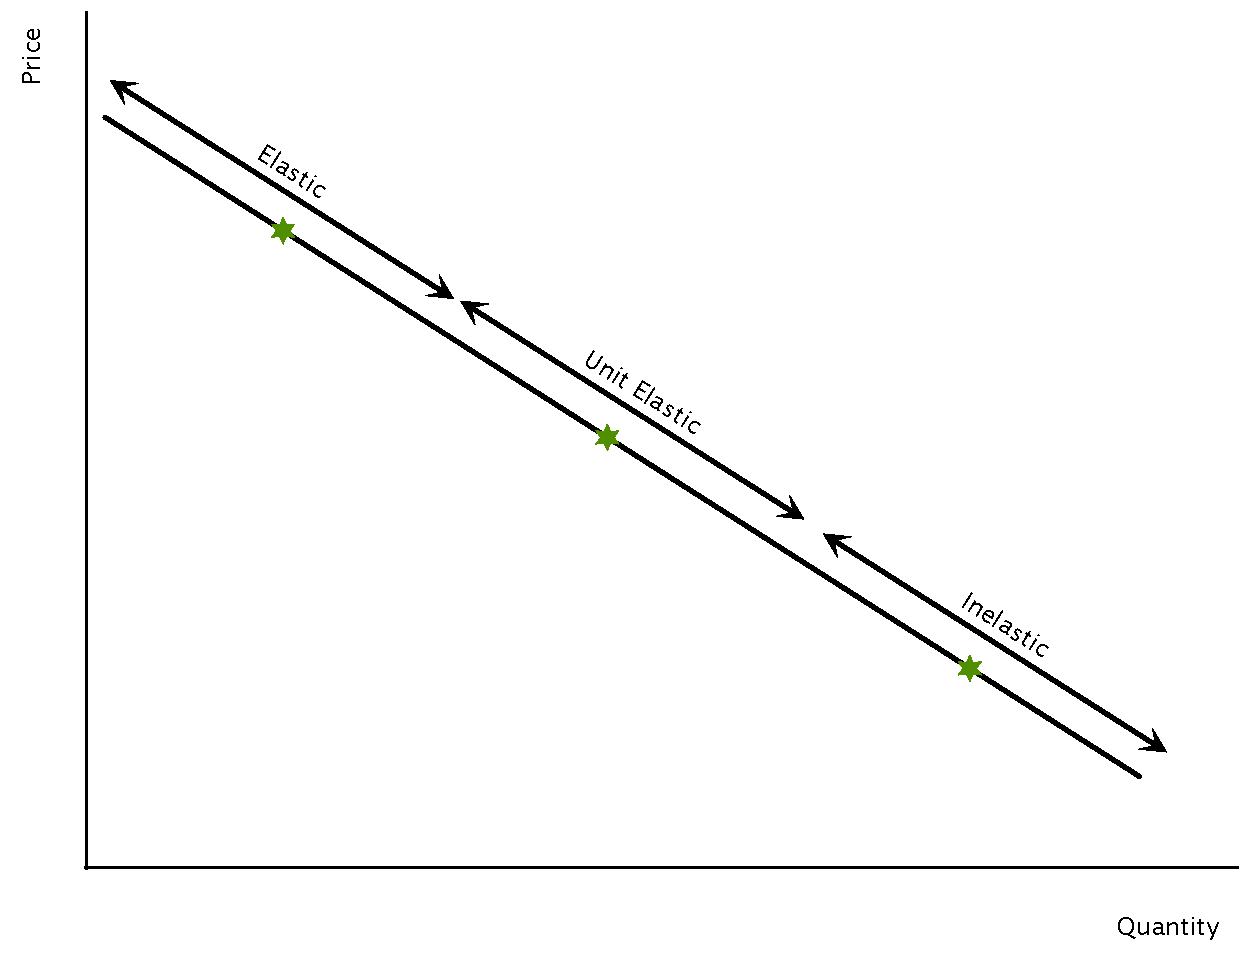
\includegraphics[scale=.25]{plot23.pdf}}
	\caption{Points along a Demand Curve}
\end{figure}
	
\end{frame}



\begin{frame}{Relative Elasticity}
	
\begin{itemize}
	\item 	Because the price elasticity of demand measures how much quantity demanded responds to changes in price, it is closely related to the slope of the demand curve. 
	\item Rearranging the equation for the price elasticity of demand, we have that
		\begin{equation*}
		|\mathcal{E}_d^p|= \Big(\frac{P_0 + P_1}{Q_0 + Q_1}\Big) \times \Big|\frac{1}{m}\Big|.
		\end{equation*}
	\item Thus, a flatter demand curve is \dd{relatively elastic} compared to a steeper curve. 
	\item Conversely, a steeper demand curve is  \dd{relatively inelastic} compared to a flatter curve.
\end{itemize}
		
\end{frame}

\begin{frame}{Relative Elasticity}

		\begin{figure}[H]
			\centering
			\caption{Comparing Demand Elasticities}
			\blank\blank\blank\blank
			\label{fig1}
			\begin{subfigure}{.5\textwidth}
				\ddp{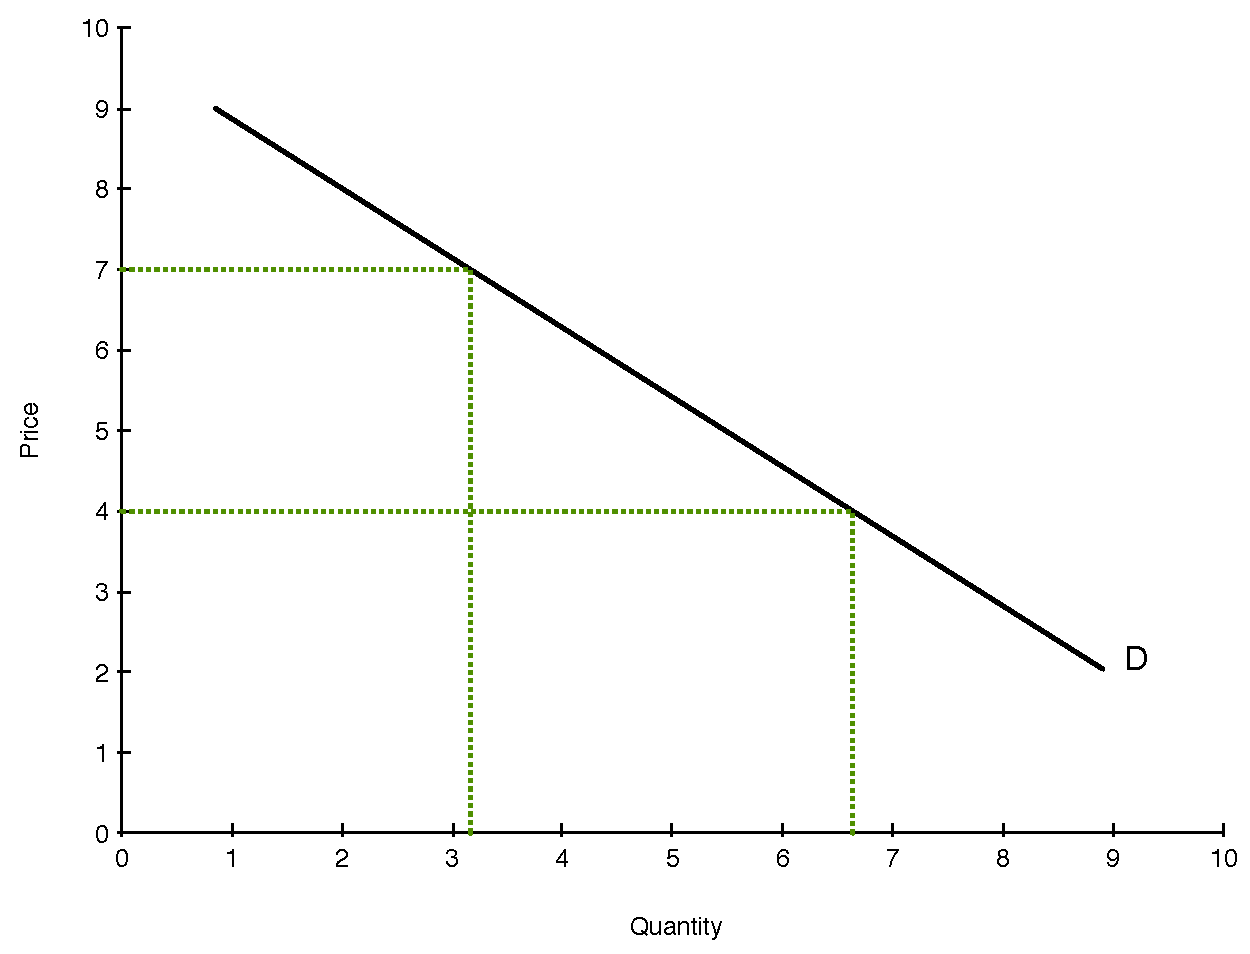
\includegraphics[scale=.25]{notes04_plot1.pdf}}
				\caption{Relatively Elastic\\ Demand Curve}
			\end{subfigure}%
			\begin{subfigure}{.5\textwidth}
				\centering
				\ddp{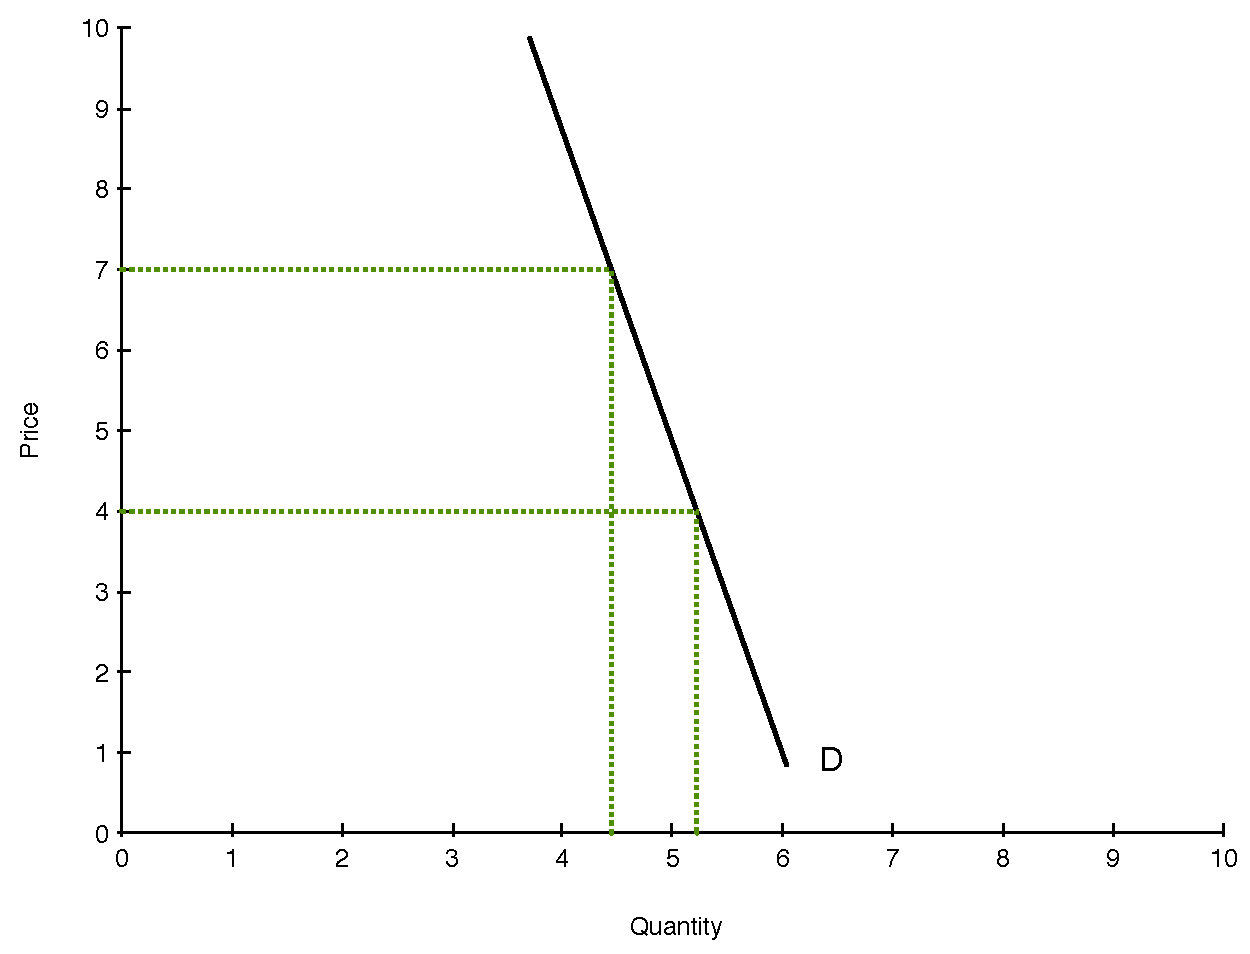
\includegraphics[scale=.25]{notes04_plot2.pdf}}
				\caption{Relatively Inelastic \\ Demand Curve}
			\end{subfigure}
		\end{figure}
	
\end{frame}

\begin{frame}{Relative Elasticity}
		\begin{figure}[H]
			\centering
			\caption{Extreme Cases}
			\blank\blank\blank\blank
			\begin{subfigure}{.5\textwidth}
			\ddp{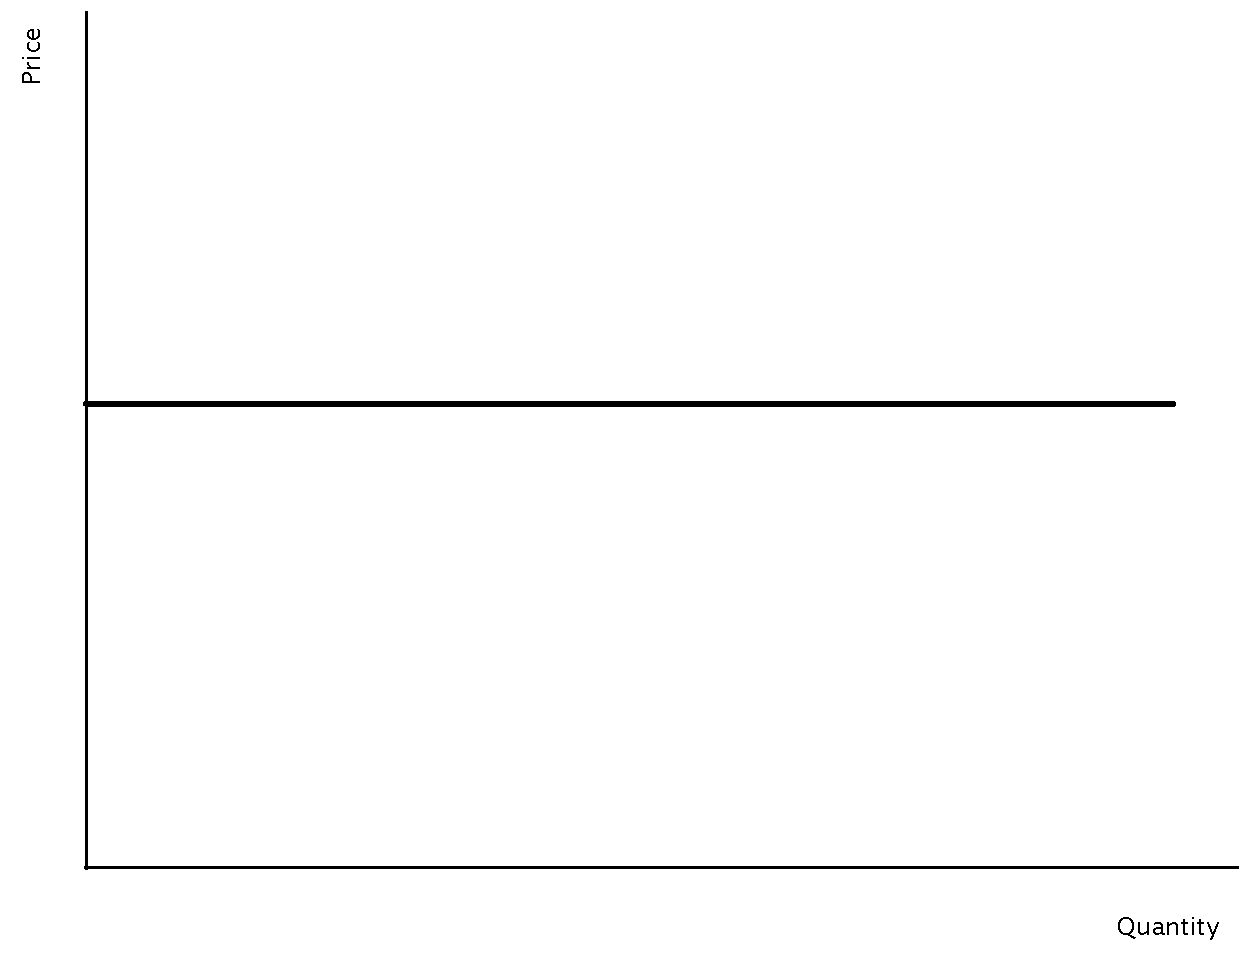
\includegraphics[scale=.25]{plot24.pdf}}
				\caption{Perfectly Elastic Demand}
			\end{subfigure}%
			\begin{subfigure}{.5\textwidth}
				\centering
				\ddp{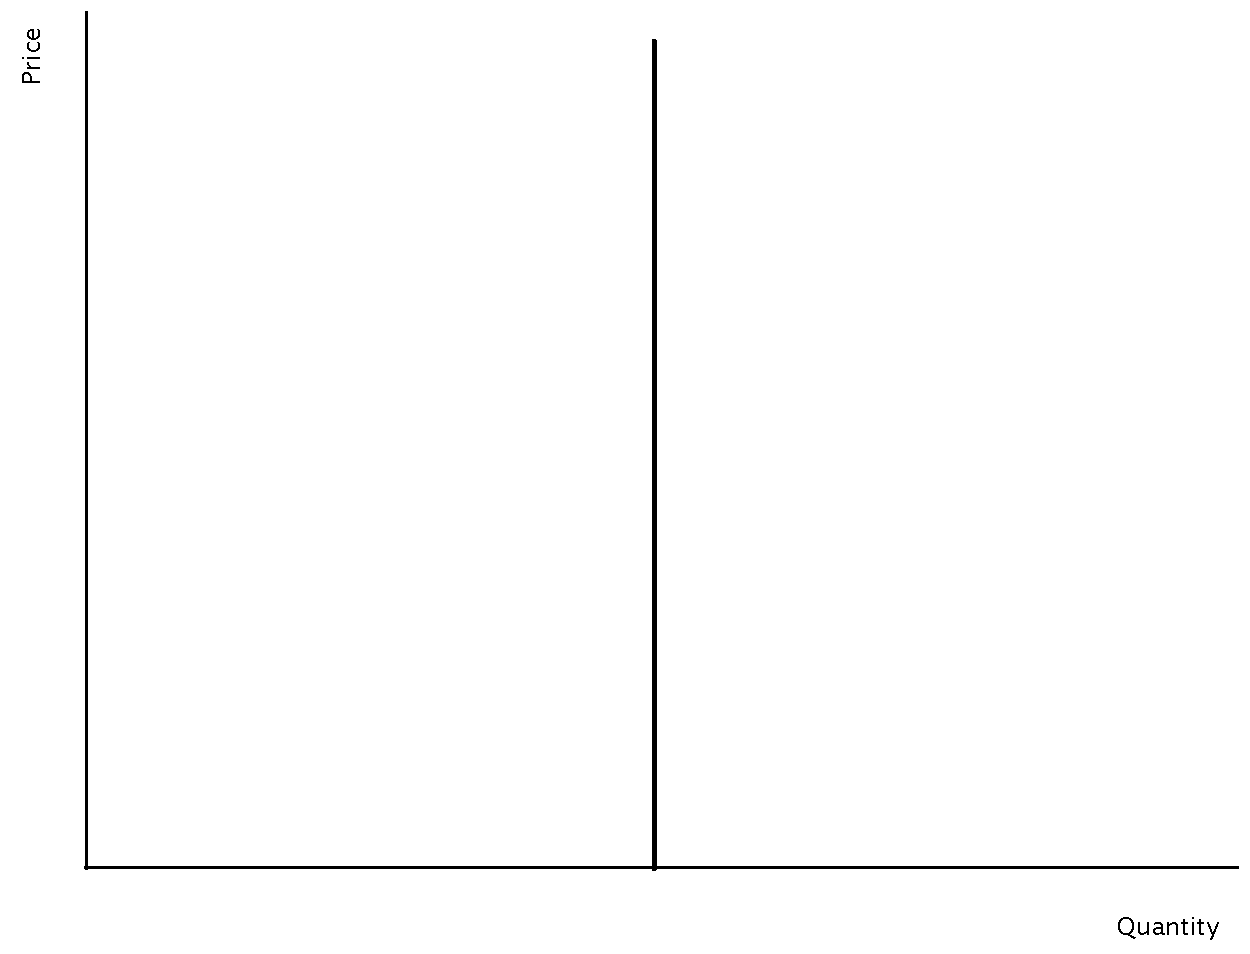
\includegraphics[scale=.25]{plot25.pdf}}
				\caption{Perfectly Inelastic Demand}
			\end{subfigure}
		\end{figure}

\end{frame}

\begin{frame}{Relative Elasticity}
	
	\begin{exmp} 
		Megan goes to her favorite coffee shop every morning and always buys one large black coffee, not matter whether there is a special or not. What is her price elasticity of demand?
	\end{exmp}

\pause	\ddp{No matter what the price is, quantity demanded does not change. Her price elasticity of demand is zero and she has a perfectly inelastic demand curve.}
	
\end{frame}

\section{Elasticity and Revenue}

\begin{frame}{Total Revenue and Price Elasticity of Demand}
\begin{itemize}
	\item \defn{Total Revenue:} The total amount paid by buyers \& received by sellers of a good. $TR = P\times Q$.
	\item As prices change, the change in total revenue depends on the elasticity of demand.
	\item 	We can write the percentage change in total revenue as \ddp{\[\%\Delta TR \approx \% \Delta P + \%\Delta Q_D\]}

	
\end{itemize}
\end{frame}

\begin{frame}{Total Revenue and Price Elasticity of Demand}

		\begin{figure}[H]
			\centering
			\ddp{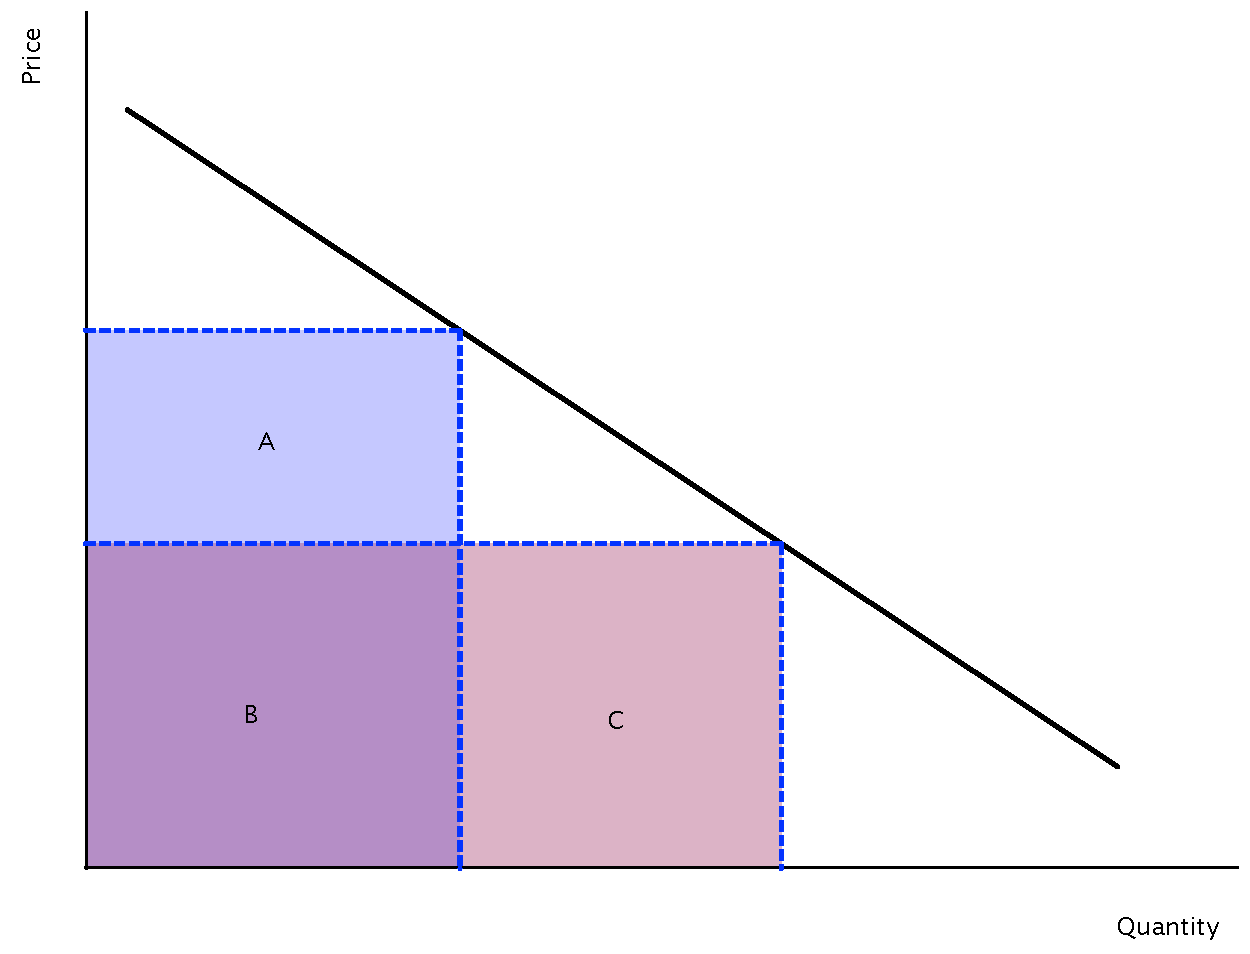
\includegraphics[scale=.25]{plot26.pdf}}
			\caption{Total Revenue}
		\end{figure}
		
\end{frame}

\begin{frame}{Total Revenue and Price Elasticity of Demand}
	
	\begin{itemize}
		\item If demand is inelastic, \dd{$|\% \Delta P| > |\%\Delta Q_D|$}. Thus, if prices rise then total revenue will \dd{increase}.
		
		\item If demand is elastic, \dd{$|\% \Delta P| < |\%\Delta Q_D|$}. Thus, if prices rise then total revenue will \dd{decrease}.
		
		
		\item If demand is unit elastic, \dd{$|\% \Delta P| = |\%\Delta Q_D|$}. Thus, total revenue will \dd{not change} when the price changes.
	\end{itemize}

		
\end{frame}


\begin{frame}{Total Revenue and Price Elasticity of Demand}

	\begin{figure}[H]
		\centering
		\caption{Comparing Demand Elasticities and Total Revenue}
		\blank\blank\blank
		\begin{subfigure}{.3\textwidth}
			\ddp{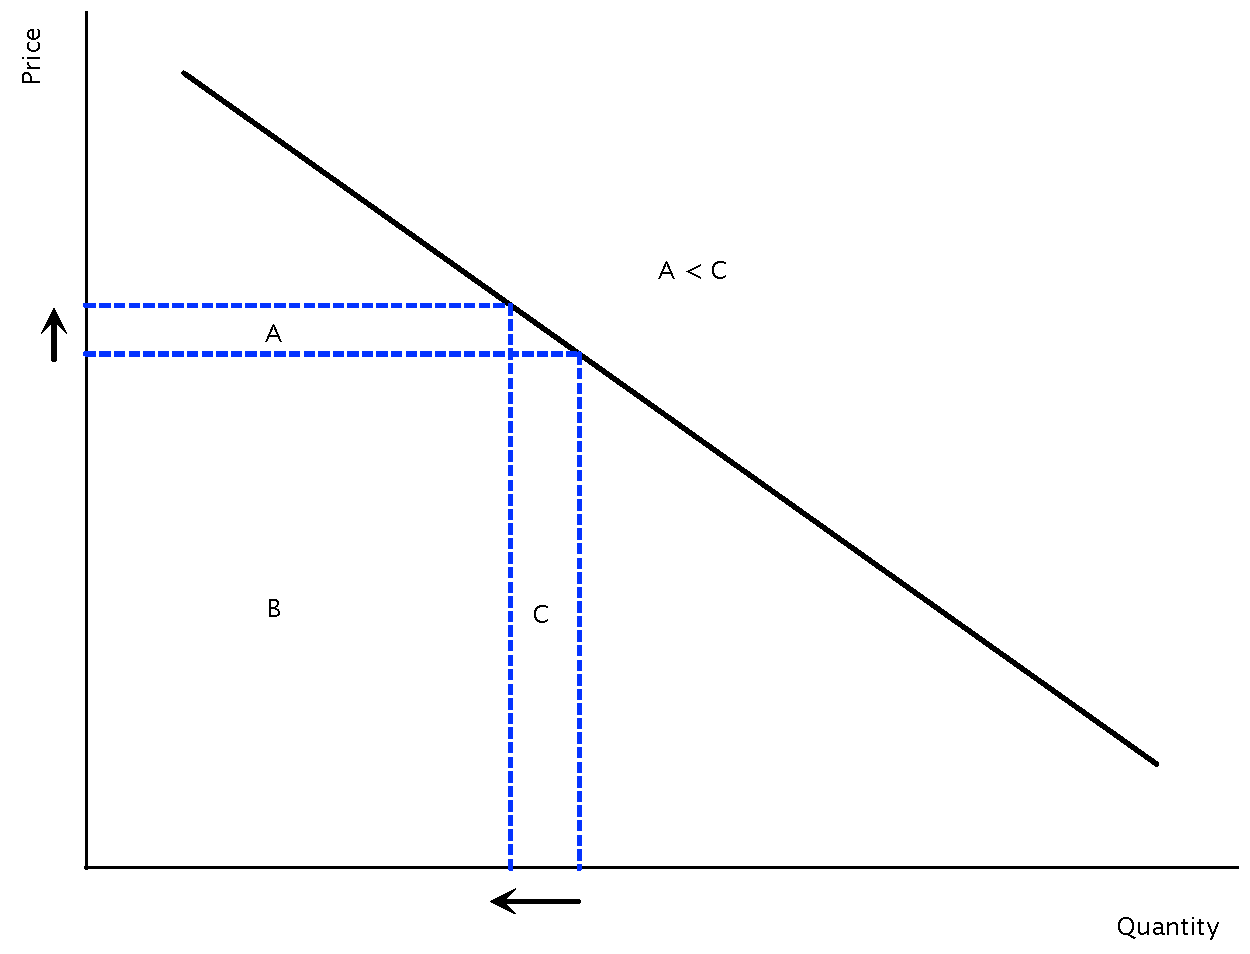
\includegraphics[scale=.18]{plot27.pdf}}
			\caption{Elastic Point}
		\end{subfigure}%
		\begin{subfigure}{.3\textwidth}
			\centering
			\ddp{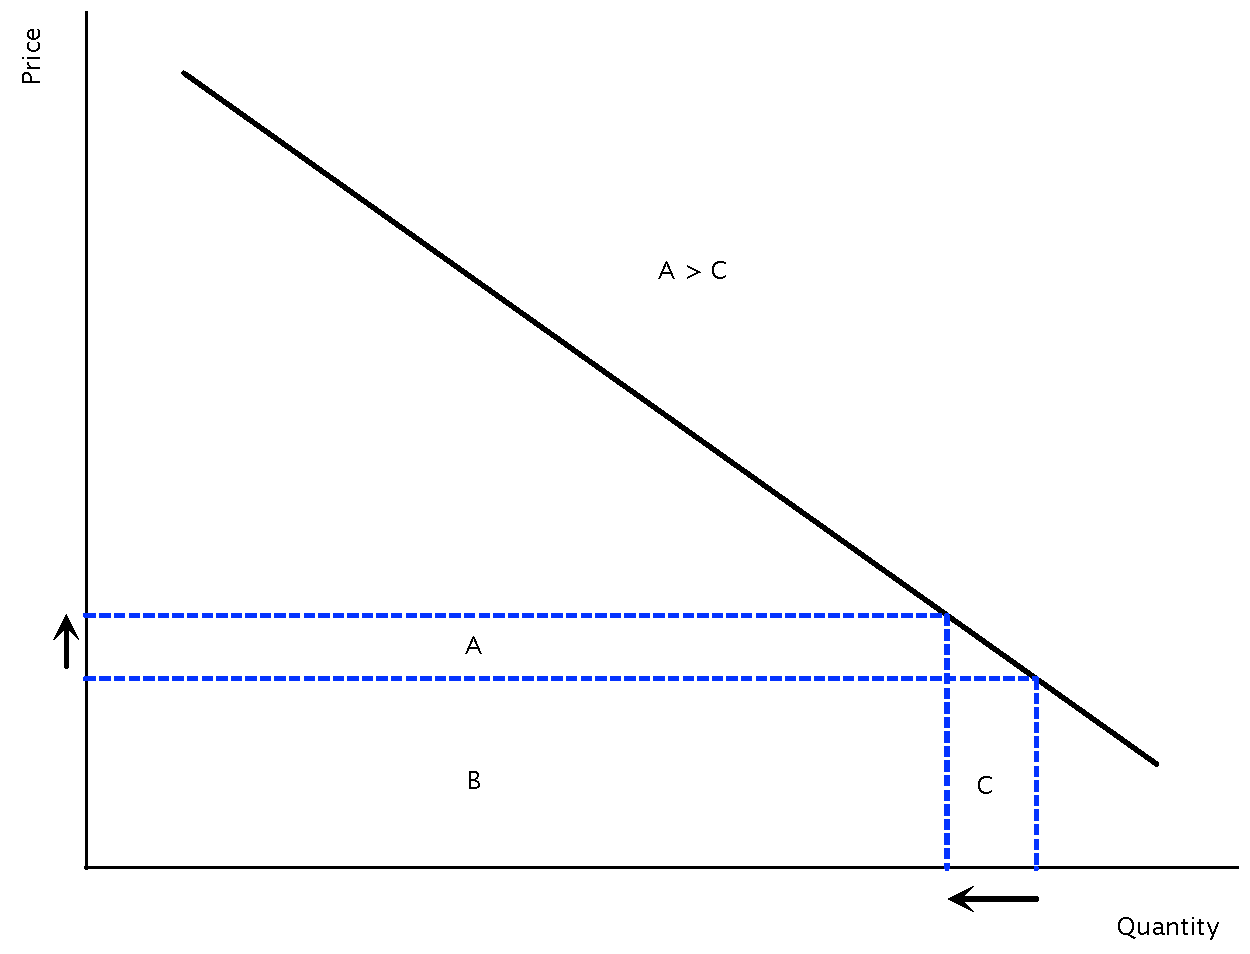
\includegraphics[scale=.18]{plot29.pdf}}
			\caption{Inelastic Point}
		\end{subfigure}
		\begin{subfigure}{.3\textwidth}
			\centering
			\ddp{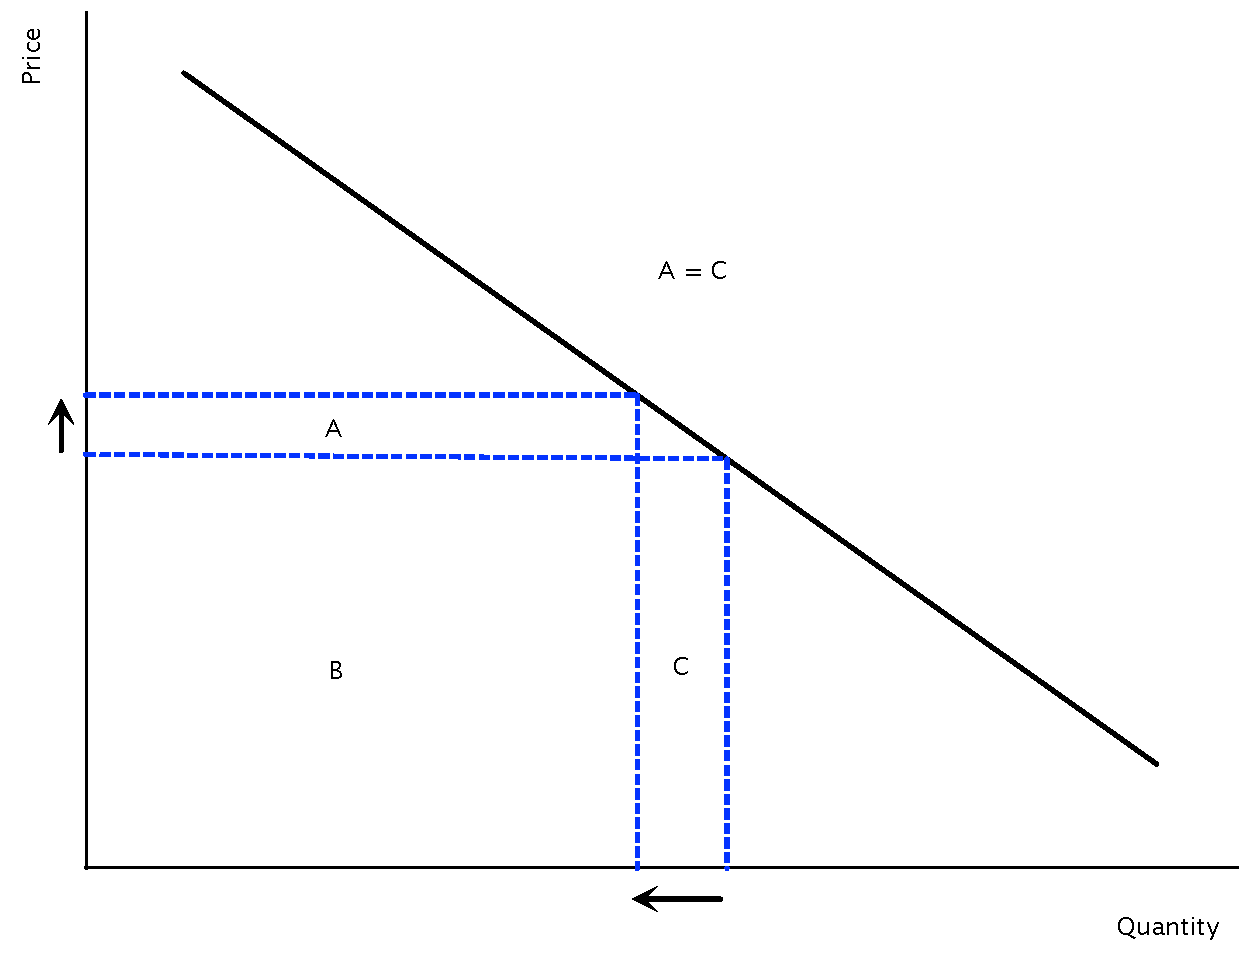
\includegraphics[scale=.18]{plot28.pdf}}
			\caption{Unit Elastic Point}
		\end{subfigure}
	\end{figure}
	
\end{frame}


\begin{frame}{Total Revenue and Price Elasticity}
		\begin{exmp} 
			The local pizza restaurant makes such great bread sticks that consumers do not respond much at all to a change in the price. If the owner is only interested in increasing revenue, he should
			
			\begin{enumerate}[(a)]
				{\setlength\itemindent{25pt} \item lower the price of bread sticks}
				{\setlength\itemindent{25pt} \item leave the price of bread sticks alone}
				{\setlength\itemindent{25pt} \item raise the price of bread sticks}
				{\setlength\itemindent{25pt} \item reduce costs}
			\end{enumerate}	
		\end{exmp}
		
	\pause	\ddp{Consumers aren't responsive to price changes, so demand is inelastic. He should increase the price of breadsticks (c).}
\end{frame}

\begin{frame}{Total Revenue and Price Elasticity}
		\begin{exmp} 
			
			Assume drug addicts pay for their addictions by stealing so that the higher the total revenue of the illegal drug industry, the higher the amount of theft.
			
			\begin{enumerate}
				\item Suppose the government cracks down on drug suppliers by imposing stiff penalties for those caught dealing drugs. How will this affect the price of illegal drugs?
				
				\item What happens to the amount of stealing if the demand for drugs is elastic? Inelastic?
			
				
				\item If instead the government pursued a policy of drug education that reduced the demand for drugs, what would be the effect on stealing? 
							
			\end{enumerate}
		\end{exmp}
	

\end{frame}

\begin{frame}[b]{Total Revenue and Price Elasticity}
		\begin{figure}[H]
			\centering
			\ddp{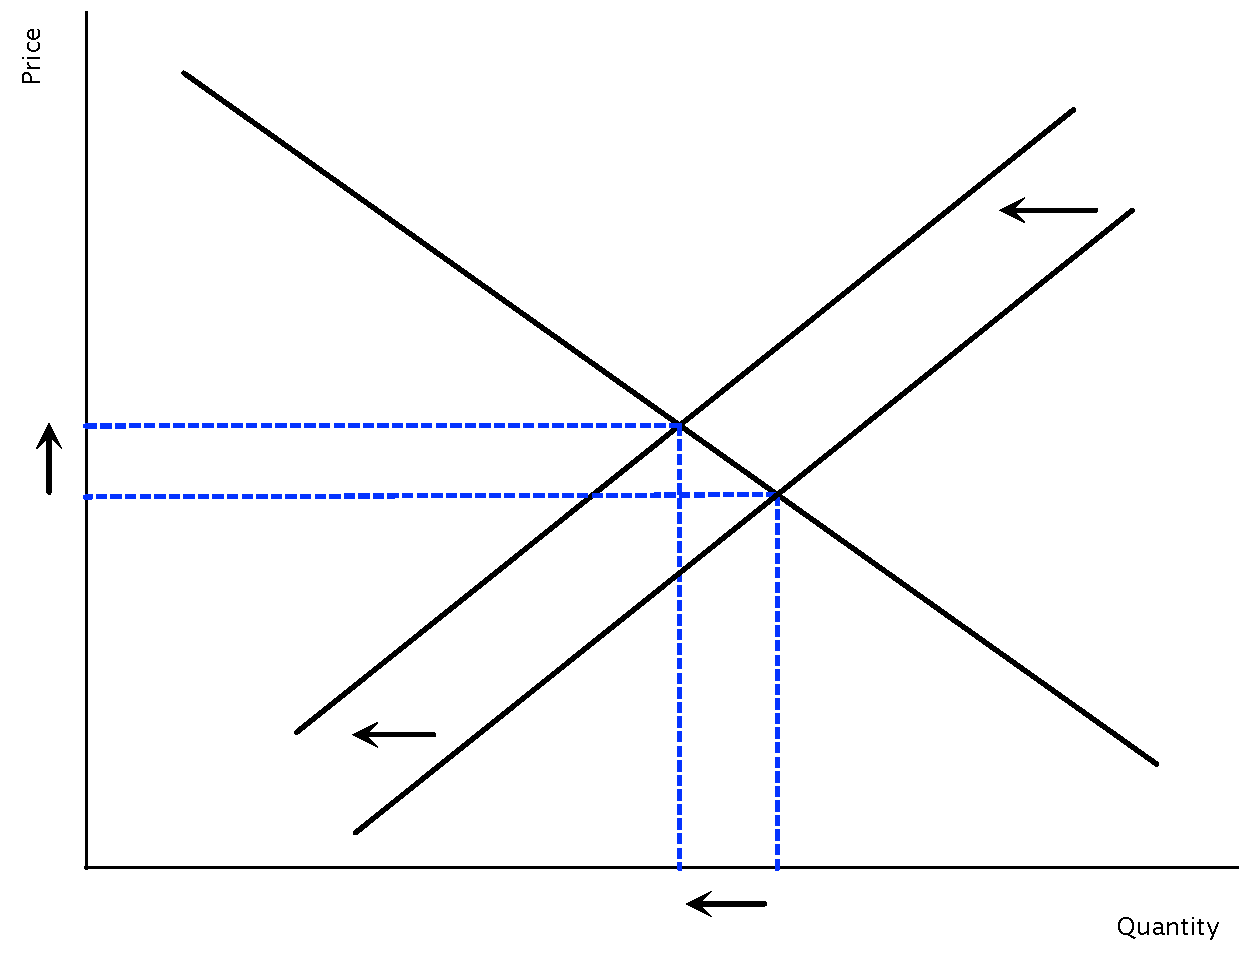
\includegraphics[scale=.25]{plot30.pdf}}
			\caption{Drug Crack Down}
		\end{figure}
		
		\ddp{The price of drugs will increase since supply decreases. The change in total revenue depends on the elasticity of demand.}
\end{frame}

\begin{frame}[b]{Total Revenue and Price Elasticity}
		\begin{figure}[H]
			\centering
			\begin{subfigure}{.5\textwidth}
				\ddp{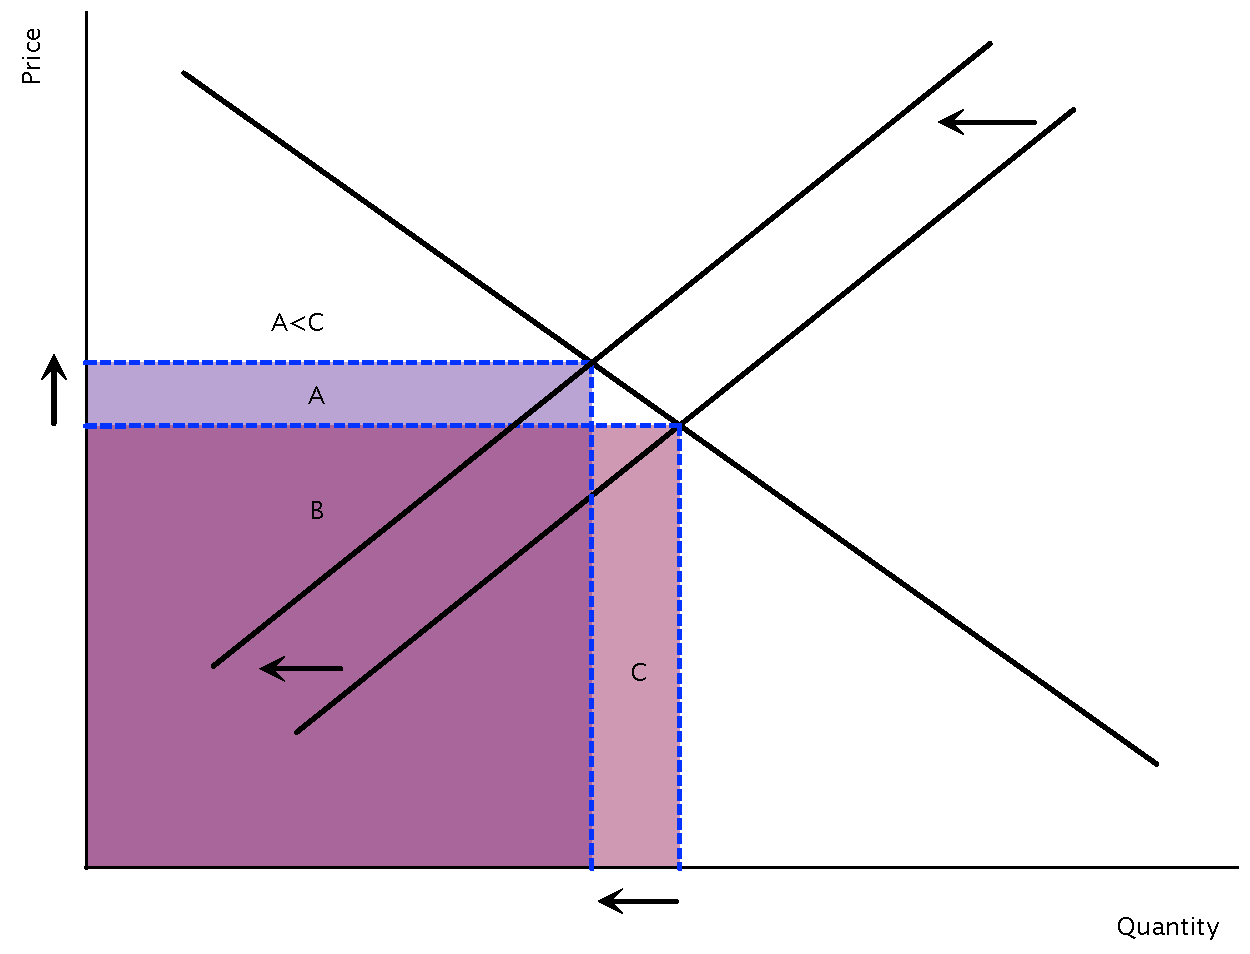
\includegraphics[scale=.25]{plot31.pdf}}
				\caption{Drug Crack Down: Elastic}
			\end{subfigure}%
			\begin{subfigure}{.5\textwidth}
				\centering
				\ddp{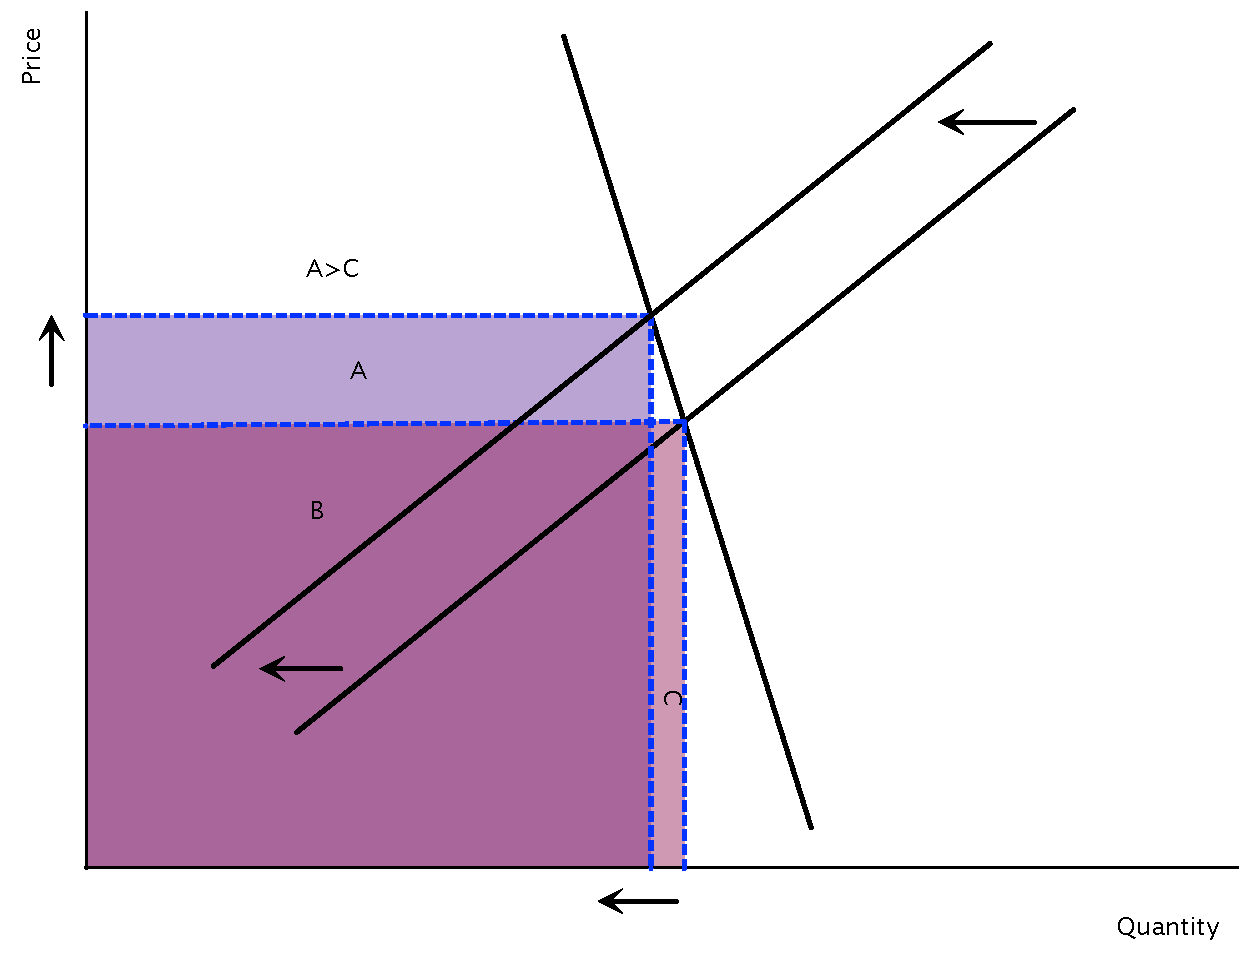
\includegraphics[scale=.25]{plot32.pdf}}
				\caption{Drug Crack Down: Inelastic}
			\end{subfigure}
		\end{figure}
		
		\ddp{In the elastic case, the amount of stealing will decrease because the decrease in quantity will outweigh the increase in price. In the inelastic case, stealing will increase since the price effect will dominate.}
\end{frame}

\begin{frame}[b]{Total Revenue and Price Elasticity}
	
	
	\begin{figure}[H]
		\centering
		\ddp{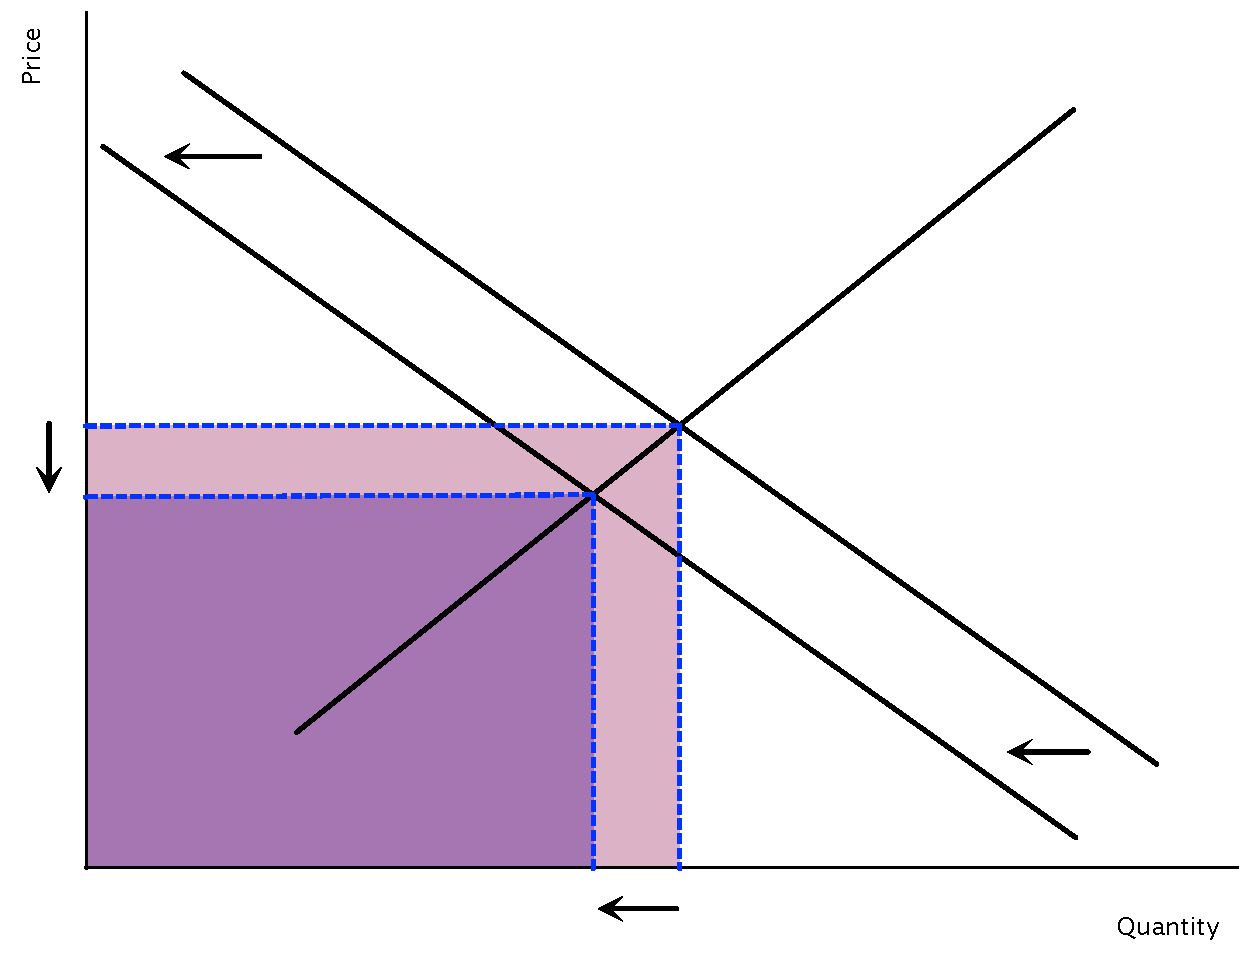
\includegraphics[scale=.25]{plot33.pdf}}
		\caption{Drug Education Policy}
	\end{figure}
	
	\ddp{The drug education policy will result in both a lower equilibrium price and quantity, which will reduce the amount of stealing.}
\end{frame}

\section{Other Elasticities}

\begin{frame}{Income Elasticity of Demand}
	\begin{itemize}
		\item \defn{Income elasticity of demand:} A measure of how much quantity demanded responds to a change in consumers' income.
		
		\[\mathcal{E}_d^I =\frac{\% \Delta Q_D}{\% \Delta I}\]

		
	\end{itemize}
\end{frame}

\begin{frame}{Income Elasticity of Demand}

		
		\begin{itemize}
			
			\item	If a good is \defn{normal}, a higher (lower) income will increase (decrease) quantity demanded. Thus,  $\mathcal{E}_d^I$ is \dd{positive} for these goods because if \dd{$\%\Delta I\gtrless  0$}, then \dd{$\%\Delta Q_D\gtrless  0$}. 
			\\
			
			\item	If a good is \defn{inferior},  a higher (lower) income will decrease (increase) quantity demanded. Thus, $\mathcal{E}_d^I$ is \dd{negative} for these goods because if \dd{$\%\Delta I\gtrless  0$}, then \dd{$\%\Delta Q_D\lessgtr  0$}. 
		\end{itemize}
		
		

\end{frame}

\begin{frame}{Cross-Price Elasticity of Demand}
	\begin{itemize}
			\item \defn{Cross-price elasticity of demand:} A measure of how much the quantity demanded of one good responds to a change in the price of another good.
			
			\[\mathcal{E}_{d_x}^{p_y} = \frac{\% \Delta Q_{D_x}}{\% \Delta P_y}\] 
	
\end{itemize}
\end{frame}

\begin{frame}{Cross-Price Elasticity of Demand}

		\begin{itemize}	
			\item	If the goods are \defn{substitutes}, an increase (decrease) in the price of one good increases (decreases) the quantity demanded of the other. Thus, $\mathcal{E}_{d_x}^{p_y}$ is \dd{positive} because if \dd{$\%\Delta P_y \gtrless  0$}, then \dd{$\%\Delta Q_{D_x}\gtrless 0$}. 
			
			\item	If the goods are \defn{complements}, an increase (decrease) in the price of one good decreases (increases) the quantity demanded of the other. Thus, $\mathcal{E}_{d_x}^{p_y}$ is \dd{negative} because if  \dd{$\%\Delta P_y\gtrless  0$}, then \dd{$\%\Delta Q_{D_x} \lessgtr  0$}.
		\end{itemize}

\end{frame}

\begin{frame}[t]
\begin{exmp} 
	\scriptsize
	Figure \ref{fig2} shows that the demand for Converse shoes has increased because average consumer incomes have increased from \$2,000 to \$4,000. What is the income elasticity of demand for Converse shoes?
\end{exmp}


	\begin{figure}[H]
	\centering
	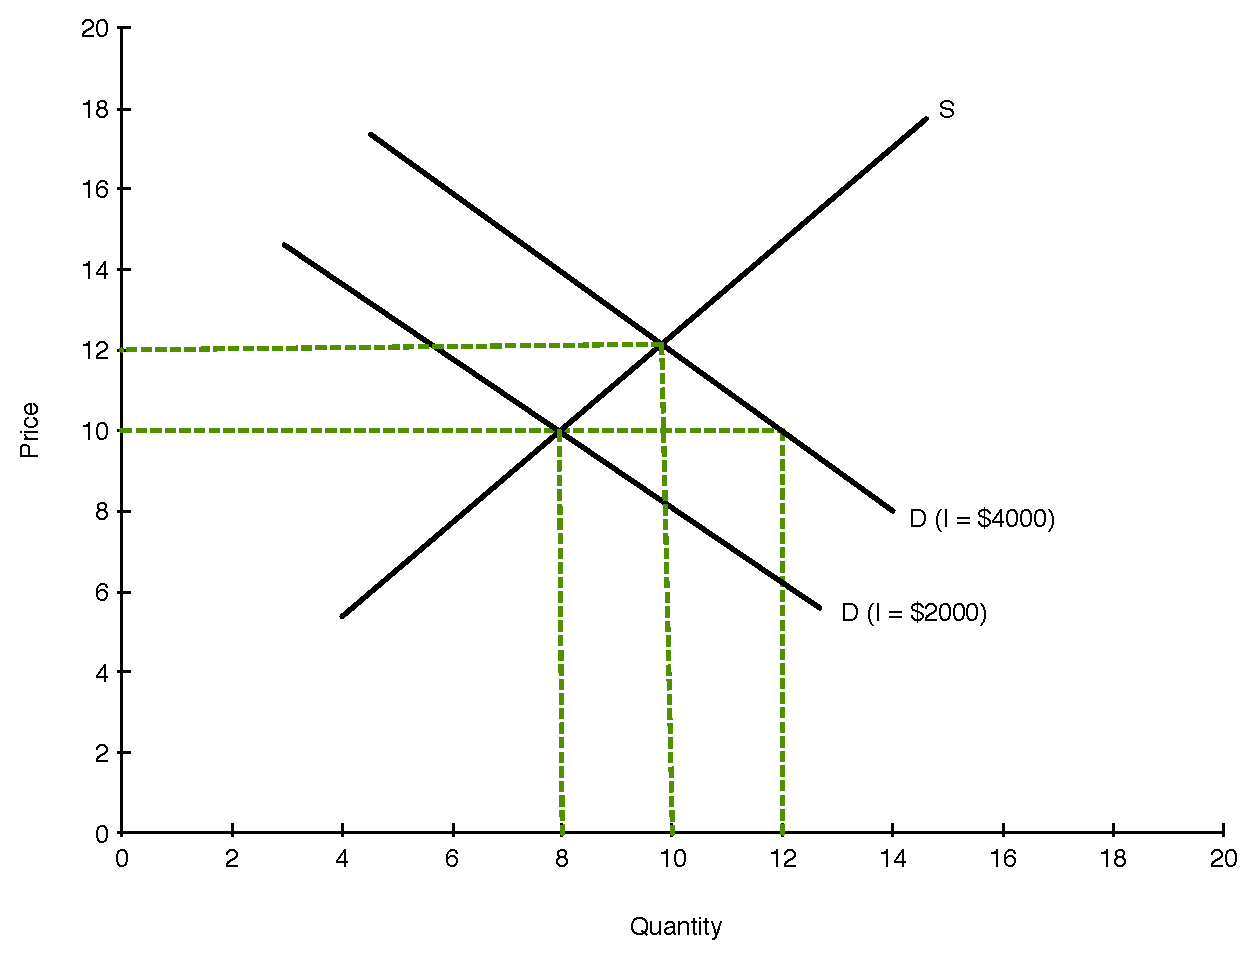
\includegraphics[scale=.25]{hw2_plot1.pdf}
	\caption{Market for Converse Shoes}
	\label{fig2}
\end{figure}

\pause
\ddp{\scriptsize  Hold the price constant at $P=\$10$ 
	\\ $\% \Delta Q_D = 12-8/10 = 40\%$ $\% \Delta I = 4000-2000/3000 = 67\%$ \\ $\mathcal{E}_d^I = .4/.67 = .60.$ This is a normal good}
\end{frame}

\begin{frame}{Price Elasticity of Supply}
	\begin{itemize}
		\item 	\defn{Price Elasticity of Supply:} A measure of how much quantity supplied responds to changes in prices of a good.
		
		
		\item The major determinant of price elasticity of supply we will examine is the time horizon. In the long run, supply is \dd{more elastic}.

	\end{itemize}
\end{frame}

\begin{frame}{Readings and Assignments}
\begin{itemize}
	\item Today: Mankiw Ch. 5
	\item Next time: Mankiw Ch. 6
	\item Problem Set 2, section 1
\end{itemize}
\end{frame}

\end{document}